% !TEX root = ./article.tex

\documentclass[spanish]{article}

\usepackage{mystyle}
\usepackage{myvars}
\usepackage{mylinearprogramming}



%-----------------------------

\begin{document}

	\maketitle % Insert title

	\thispagestyle{fancy} % All pages have headers and footers


%-----------------------------
%	ABSTRACT
%-----------------------------

	\begin{abstract}
		\noindent En este documento se realiza una descripción acerca del \emph{problema del viajante} (TSP), que consiste en la búsqueda del camino más corto que permita visitar un conjunto de nodos. Además se proporcionan distintas formulaciones para dicho problema así como un conjunto de heurísticas aproximadas que permiten su resolución de manera mucho menos costosa. También se presenta la descripción de la variante del \emph{problema del viajante con ventana de tiempo} (TSPTW), que se caracteriza por exigir que la visita de un determinado nodo se realice dentro de un intervalo temporal prefijado. Por último, se presentan las soluciones de distintos conjuntos de datos resultas mediantes las estrategias descritas en el documento.
	\end{abstract}

%-----------------------------
%	TEXT
%-----------------------------

	\section{Introducción}
	\label{sec:intro}

		\paragraph{}
		[TODO ]

	\section{Problema del Viajante (TSP)}

		\paragraph{}
		[TODO ]

		\begin{eqfloat}
			\begin{equation}
				\begin{array}{ll@{}ll}
					\text{Minimizar}	& \displaystyle\sum\limits_{i = 1}^{n}\sum\limits_{j}^{n} & d_{ij}x_{ij} &\\
					\text{sujeto a}		& \displaystyle\sum\limits_{i = 1}^{n}	&	x_{ij} 	= 1,  & \forall j \in \{1,...,n\}\\
														& \displaystyle\sum\limits_{j = 1}^{n}	&	x_{ij} 	= 1,  & \forall i \in \{1,...,n\}\\
														& \displaystyle\sum\limits_{i \in S, j \not\in S}	&	x_{ij} 	\geq 1,  & \forall S \subset N / S \neq \emptyset, S \neq N \\
														&                               &	x_{ij} \in \{0,1\}, 	& \forall i,j \in \{1,...,n\}
				\end{array}
			\end{equation}
			\caption{Formulación estándar para el \emph{problema del viajante (TSP)}.}
			\label{eq:tsp_basic}
		\end{eqfloat}

		\subsection{Estrategia Exacta}

			\paragraph{}
			[TODO ]

			\subsection{Formulación de Tucker-Miller}

				\paragraph{}
				[TODO ]

				\begin{eqfloat}
					\begin{equation}
						\begin{array}{ll@{}ll}
							\text{Minimizar}	& \displaystyle\sum\limits_{i = 1}^{n}\sum\limits_{j}^{n} & d_{ij}x_{ij} &\\
							\text{sujeto a}		& \displaystyle\sum\limits_{i = 1}^{n}	&	x_{ij} 	= 1,  & \forall j \in \{1,...,n\} \\
																& \displaystyle\sum\limits_{j = 1}^{n}	&	x_{ij} 	= 1,  & \forall i \in \{1,...,n\} \\
																& 				&	u_i - u_j + n x_{ij}	\leq n-1,  & \forall i, j \in \{2,...,n\}, i \neq j \\
																&                               &	u_{i} \in \{2,...,n\}, 		& \forall i \in \{2,...,n\} \\
																&                               &	u_{1}  = 1, 	& \\
																&                               &	x_{ij} \in \{0,1\}, 	& \forall i,j \in \{1,...,n\}
						\end{array}
					\end{equation}
					\caption{Formulación de Tucker-Miller para el \emph{problema del viajante (TSP)}.}
					\label{eq:tsp_tm}
				\end{eqfloat}

			\subsection{Formulación de Redes}

				\paragraph{}
				[TODO ]

				\begin{eqfloat}
					\begin{equation}
						\begin{array}{ll@{}ll}
							\text{Minimizar}	& \displaystyle\sum\limits_{i = 1}^{n}\sum\limits_{j}^{n} & d_{ij}x_{ij} &\\
							\text{sujeto a}		& \displaystyle\sum\limits_{i = 1}^{n}	&	x_{ij} 	= 1,  & \forall j \in \{1,...,n\}\\
																& \displaystyle\sum\limits_{j = 1}^{n}	&	x_{ij} 	= 1,  & \forall i \in \{1,...,n\}\\
																& \displaystyle\sum\limits_{j = 1}^n	y_{ij} - &\displaystyle\sum\limits_{j = 1}^n	y_{ji} = b_{i},  & \forall i \in \{1,...,n\} \\
																&                               &	y_{ij}  \leq (n-1)x_{ij}, 	&  \forall i,j \in \{1,...,n\}\\
																&                               &	b_{1}  = n - 1, 	& \\
																&                               &	b_{i} = -1, 		& \forall i \in \{2,...,n\} \\
																&                               &	y_{ij} \geq 0, 		& \forall i,j \in \{1,...,n\} \\
																&                               &	x_{ij} \in \{0,1\}, 	& \forall i,j \in \{1,...,n\}
						\end{array}
					\end{equation}
					\caption{Formulación de Redes para els \emph{problema del viajante (TSP)}.}
					\label{eq:tsp_redes}
				\end{eqfloat}


		\subsection{Estrategia Entorno más Cercano}

			\paragraph{}
			[TODO ]

			\begin{figure}
	      \centering
	      \BVerbatimInput{code/tsp-greedy.pseudo}
	      \caption{Heurística del \emph{Entorno más Cercano}}
	      \label{code:tsp-greedy}
	    \end{figure}

		\subsection{Estrategia 2-OPT}

			\paragraph{}
			[TODO ]

			\begin{figure}
	      \centering
	      \BVerbatimInput{code/tsp-2-opt.pseudo}
	      \caption{Heurística \emph{2-opt}}
	      \label{code:tsp-2-opt}
	    \end{figure}

		\subsection{Estrategia GRASP}

			\paragraph{}
			[TODO ]

			\begin{figure}
				\centering
				\BVerbatimInput{code/tsp-grasp.pseudo}
				\caption{Heurística \emph{GRASP}}
				\label{code:tsp-grasp}
			\end{figure}

		\subsection{Estrategia Simulated Anneling}

			\paragraph{}
			[TODO ]

			\begin{figure}
	      \centering
	      \BVerbatimInput{code/tsp-simulated-anneling.pseudo}
				\caption{Heurística \emph{Simulated Anneling}}
	      \label{code:tsp-simulated-anneling}
	    \end{figure}

	\section{Problema del Viajante con Ventana de Tiempo (TSPTW)}

		\paragraph{}
		[TODO ]

		\begin{eqfloat}
			\begin{equation}
				\begin{array}{ll@{}ll}
					\text{Minimizar}	& \displaystyle\sum\limits_{i = 1}^{n}\sum\limits_{j}^{n} & d_{ij}x_{ij} &\\
					\text{sujeto a}		& \displaystyle\sum\limits_{i = 1}^{n}	&	x_{ij} 	= 1,  & \forall j \in \{1,...,n\} \\
														& \displaystyle\sum\limits_{j = 1}^{n}	&	x_{ij} 	= 1,  & \forall i \in \{1,...,n\} \\
														& 				&	\beta_{i} + d_{ij} - M(1-x_{ij}) \leq \beta_{j},  & \forall i, j \in \{1,...,n\}, j \neq 1 \\
														& 				&	u_i - u_j + n x_{ij}	\leq n-1,  & \forall i, j \in \{2,...,n\}, i \neq j \\
														&                               &	u_{i} \in \{2,...,n\}, 		& \forall i \in \{2,...,n\} \\
														&                               &	u_{1}  = 1, 	& \\
														&                               &	a_{i} \leq \beta_{i}, 		& \forall i \in \{1,...,n\} \\
														&                               &	\beta_{i} \leq b_{i}, 		& \forall i \in \{1,...,n\} \\
														&                               &	x_{ij} \in \{0,1\}, 	& \forall i,j \in \{1,...,n\}
				\end{array}
			\end{equation}
			\caption{Formulación de Tucker-Miller para el \emph{problema del viajante con ventana de tiempo (TSPTW)}.}
			\label{eq:tsp_tm}
		\end{eqfloat}

	\section{Resolución de Problemas}

		\paragraph{}
		En esta sección se presentan los resultados obtenidos tras resolver el problema del viajante (TSP) con distintos conjuntos de datos de entrada. Dichos resultados se han agrupado por problema en lugar de por estrategia de resolución, lo cual permite comparar de manera más simple cada una de ellas. En algunos casos estos conjuntos de datos se corresponden con coordenadas cartesianas, para lo cual es necesario calcular la distancias entre cada par de puntos, lo que permite realizar una representación gráfica de la solución. Sin embargo, en otros casos tan solo se suministran las distancias, por lo que la representación gráfica no es posible. Por último, se resuelven dos problemas con ventana de tiempo (TSPTW) de manera exacta, para el cual se suministran además los puntos de inicio y fin permitidos para visitar cada nodo.

		\subsection{burma14}

			\paragraph{}
			El conjunto de datos está formado por las coordenadas de $14$ nodos (por lo que es necesario calcular las distancias previamente). En este caso se resuelve de manera exacta mediante la formulación de \emph{Tucker-Miller} y la de \emph{Redes}. En la tabla \ref{table:sol-burma14} se muestran los resultados de forma numérica mientras que en la figura \ref{fig:sol-burma14} se muestra la representación gráfica. Tal y como se puede apreciar ambas soluciones son óptimas, sin embargo proporcionan caminos distintos

			\begin{table}[H]
				\centering
				\begin{tabu}{ | c | c | p{.65\linewidth} |}
					\hline
					\bfseries Método & \bfseries Distancia & \bfseries Camino
					\csvreader[head to column names]{../results/csv/results-burma14.csv}{}
					{\\\hline\method&\distance&\path}
					\\\hline
				\end{tabu}
				\caption{Soluciones para el conjunto de datos \emph{burma14}}
				\label{table:sol-burma14}
			\end{table}

			\begin{figure}[h]
				\centering
				\begin{subfigure}{.4\textwidth}
					\centering
					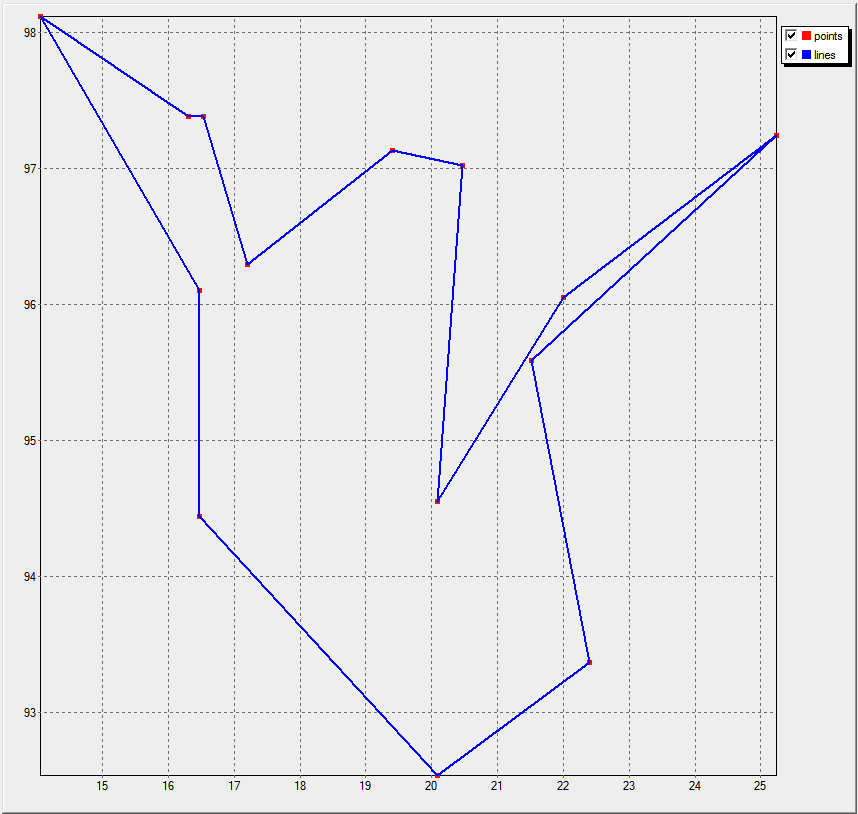
\includegraphics[width=\linewidth]{results-burma14-tm}
					\caption{Solución \emph{Exacta (TM)}}
				\end{subfigure} \
				\begin{subfigure}{.4\textwidth}
					\centering
					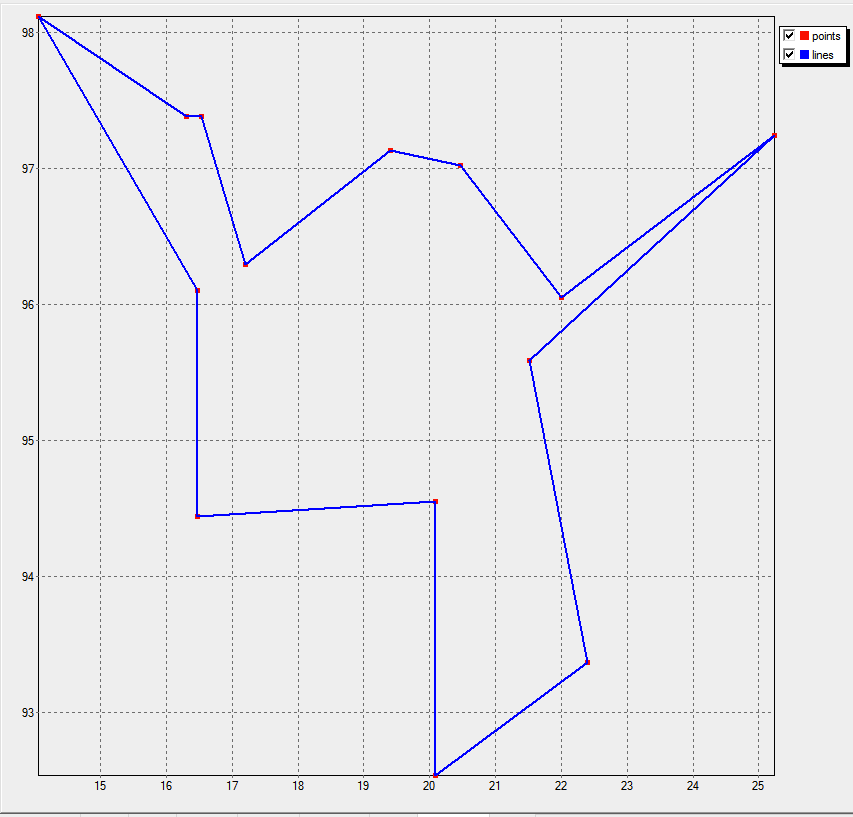
\includegraphics[width=\linewidth]{results-burma14-redes}
					\caption{Solución \emph{Entorno más Cercano (Redes)}}
				\end{subfigure}
				\caption{Representación gráfica de las distintas soluciones para el conjunto de datos \emph{burma14}}
				\label{fig:sol-burma14}
			\end{figure}


		\subsection{br17}

			\paragraph{}
			El conjunto de datos está formado por la matriz de distancias de $17$ nodos. En este caso se resuelve de manera exacta mediante la formulación de \emph{Tucker-Miller} y la de \emph{Redes}. Al igual que en el caso anterior, ambas soluciones son óptimas, sin embargo proporcionan caminos distintos. Los resultados se muestran en la tabla \ref{table:sol-br17}.

			\begin{table}[H]
				\centering
				\begin{tabu}{ | c | c | p{.65\linewidth} |}
					\hline
					\bfseries Método & \bfseries Distancia & \bfseries Camino
					\csvreader[head to column names]{../results/csv/results-br17.csv}{}
					{\\\hline\method&\distance&\path}
					\\\hline
				\end{tabu}
				\caption{Soluciones para el conjunto de datos \emph{br17}}
				\label{table:sol-br17}
			\end{table}

		\subsection{n21\_1}

			\paragraph{}
			El conjunto de datos está formado por la matriz de distancias de $21$ nodos. En este caso se ha resulto de manera exacta mediante la formulación de \emph{Tucker-Miller} y de manera aproximada mediante heurísticas \emph{Entorno más Cercano}, \emph{2-opt}, \emph{GRASP} y \emph{Simulated Anneling}. Los resultados se muestran en la tabla \ref{table:sol-n21_1}.

			\begin{table}[H]
				\centering
				\begin{tabu}{ | c | c | p{.65\linewidth} |}
					\hline
			   	\bfseries Método & \bfseries Distancia & \bfseries Camino
			    \csvreader[head to column names]{../results/csv/results-n21_1.csv}{}
			    {\\\hline\method&\distance&\path}
					\\\hline
		    \end{tabu}
				\caption{Soluciones para el conjunto de datos \emph{n21\_1}}
				\label{table:sol-n21_1}
			\end{table}

		\subsection{n21\_2}

			\paragraph{}
			El conjunto de datos está formado por la matriz de distancias de $21$ nodos. En este caso se ha resulto de manera exacta mediante la formulación de \emph{Tucker-Miller} y de manera aproximada mediante heurísticas \emph{Entorno más Cercano}, \emph{2-opt}, \emph{GRASP} y \emph{Simulated Anneling}. Los resultados se muestran en la tabla \ref{table:sol-n21_2}.

			\begin{table}[H]
				\centering
				\begin{tabu}{ | c | c | p{.65\linewidth} |}
					\hline
			   	\bfseries Método & \bfseries Distancia & \bfseries Camino
			    \csvreader[head to column names]{../results/csv/results-n21_2.csv}{}
			    {\\\hline\method&\distance&\path}
					\\\hline
		    \end{tabu}
				\caption{Soluciones para el conjunto de datos \emph{n21\_2}}
				\label{table:sol-n21_2}
			\end{table}

		\subsection{n21\_3}

			\paragraph{}
			El conjunto de datos está formado por la matriz de distancias de $21$ nodos. En este caso se ha resulto de manera exacta mediante la formulación de \emph{Tucker-Miller} y de manera aproximada mediante heurísticas \emph{Entorno más Cercano}, \emph{2-opt}, \emph{GRASP} y \emph{Simulated Anneling}. Los resultados se muestran en la tabla \ref{table:sol-n21_3}.

			\begin{table}[H]
				\centering
				\begin{tabu}{ | c | c | p{.65\linewidth} |}
					\hline
			   	\bfseries Método & \bfseries Distancia & \bfseries Camino
			    \csvreader[head to column names]{../results/csv/results-n21_3.csv}{}
			    {\\\hline\method&\distance&\path}
					\\\hline
		    \end{tabu}
				\caption{Soluciones para el conjunto de datos \emph{n21\_3}}
				\label{table:sol-n21_3}
			\end{table}

		\subsection{n21\_4}

			\paragraph{}
			El conjunto de datos está formado por la matriz de distancias de $21$ nodos. En este caso se ha resulto de manera exacta mediante la formulación de \emph{Tucker-Miller} y de manera aproximada mediante heurísticas \emph{Entorno más Cercano}, \emph{2-opt}, \emph{GRASP} y \emph{Simulated Anneling}. Los resultados se muestran en la tabla \ref{table:sol-n21_4}.

			\begin{table}[H]
				\centering
				\begin{tabu}{ | c | c | p{.65\linewidth} |}
					\hline
			   	\bfseries Método & \bfseries Distancia & \bfseries Camino
			    \csvreader[head to column names]{../results/csv/results-n21_4.csv}{}
			    {\\\hline\method&\distance&\path}
					\\\hline
		    \end{tabu}
				\caption{Soluciones para el conjunto de datos \emph{n21\_4}}
				\label{table:sol-n21_4}
			\end{table}

		\subsection{n21\_5}

			\paragraph{}
			El conjunto de datos está formado por la matriz de distancias de $21$ nodos. En este caso se ha resulto de manera exacta mediante la formulación de \emph{Tucker-Miller} y de manera aproximada mediante heurísticas \emph{Entorno más Cercano}, \emph{2-opt}, \emph{GRASP} y \emph{Simulated Anneling}. Los resultados se muestran en la tabla \ref{table:sol-n21_5}.

			\begin{table}[H]
				\centering
				\begin{tabu}{ | c | c | p{.65\linewidth} |}
					\hline
			   	\bfseries Método & \bfseries Distancia & \bfseries Camino
			    \csvreader[head to column names]{../results/csv/results-n21_5.csv}{}
			    {\\\hline\method&\distance&\path}
					\\\hline
		    \end{tabu}
				\caption{Soluciones para el conjunto de datos \emph{n21\_5}}
				\label{table:sol-n21_5}
			\end{table}

		\subsection{tsp\_60\_1}

			\paragraph{}
			El conjunto de datos está formado por las coordenadas de $60$ nodos (por lo que es necesario calcular las distancias previamente). En este caso se ha resulto de manera exacta mediante la formulación de \emph{Tucker-Miller} y de manera aproximada mediante heurísticas \emph{Entorno más Cercano}, \emph{2-opt}, \emph{GRASP} y \emph{Simulated Anneling}. En la tabla \ref{table:sol-tsp_60_1} se muestran los resultados de forma numérica mientras que en la figura \ref{fig:sol-tsp_60_1} se muestra la representación gráfica.

			\begin{table}[H]
				\centering
				\begin{tabu}{ | c | c | p{.65\linewidth} |}
					\hline
			   	\bfseries Método & \bfseries Distancia & \bfseries Camino
			    \csvreader[head to column names]{../results/csv/results-tsp_60_1.csv}{}
			    {\\\hline\method&\distance&\path}
					\\\hline
		    \end{tabu}
				\caption{Soluciones para el conjunto de datos \emph{tsp\_60\_1}}
				\label{table:sol-tsp_60_1}
			\end{table}


			\begin{figure}[h]
				\centering
				\begin{subfigure}{.4\textwidth}
					\centering
					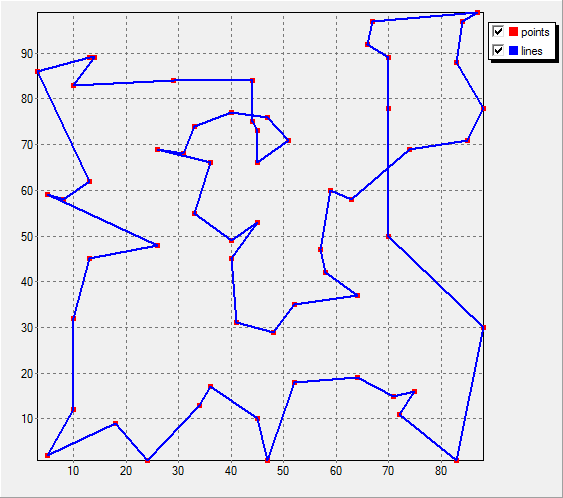
\includegraphics[width=\linewidth]{results-tsp_60_1-exact}
					\caption{Solución \emph{Exacta}}
				\end{subfigure} \
				\begin{subfigure}{.4\textwidth}
					\centering
					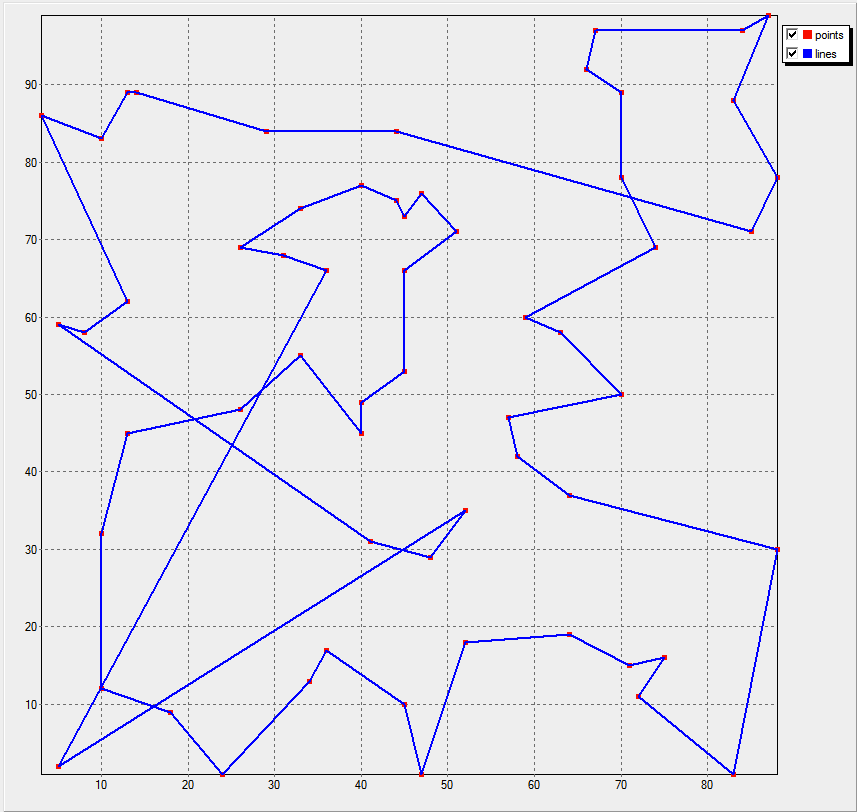
\includegraphics[width=\linewidth]{results-tsp_60_1-greedy}
					\caption{Solución \emph{Entorno más Cercano}}
				\end{subfigure} \\
				\begin{subfigure}{.4\textwidth}
					\centering
					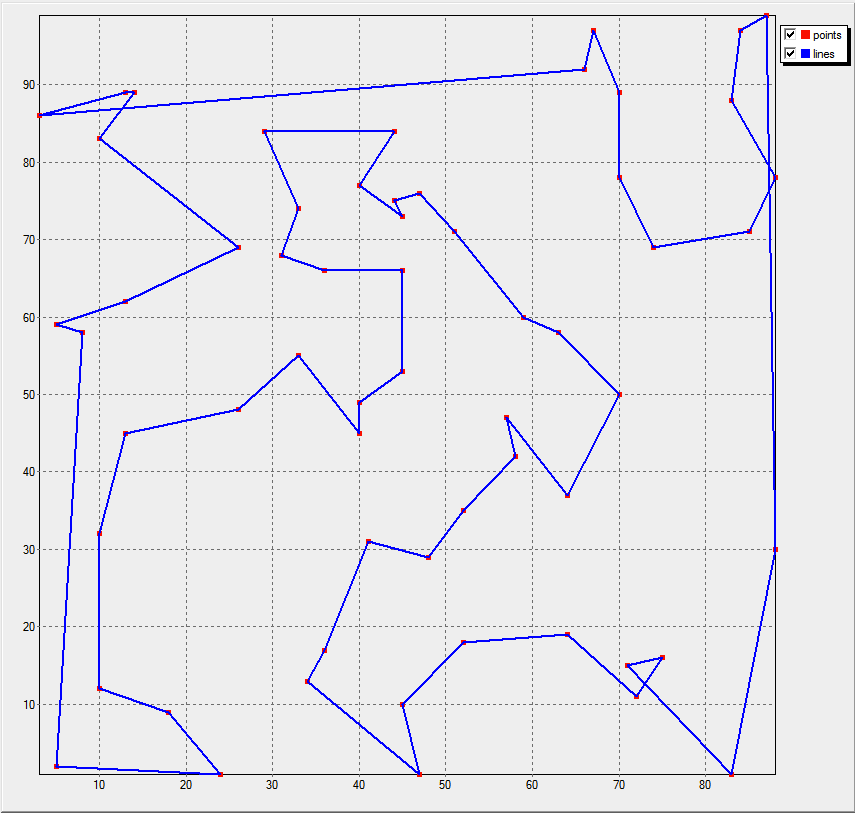
\includegraphics[width=\linewidth]{results-tsp_60_1-opt}
					\caption{Solución \emph{2-opt}}
				\end{subfigure} \
				\begin{subfigure}{.4\textwidth}
					\centering
					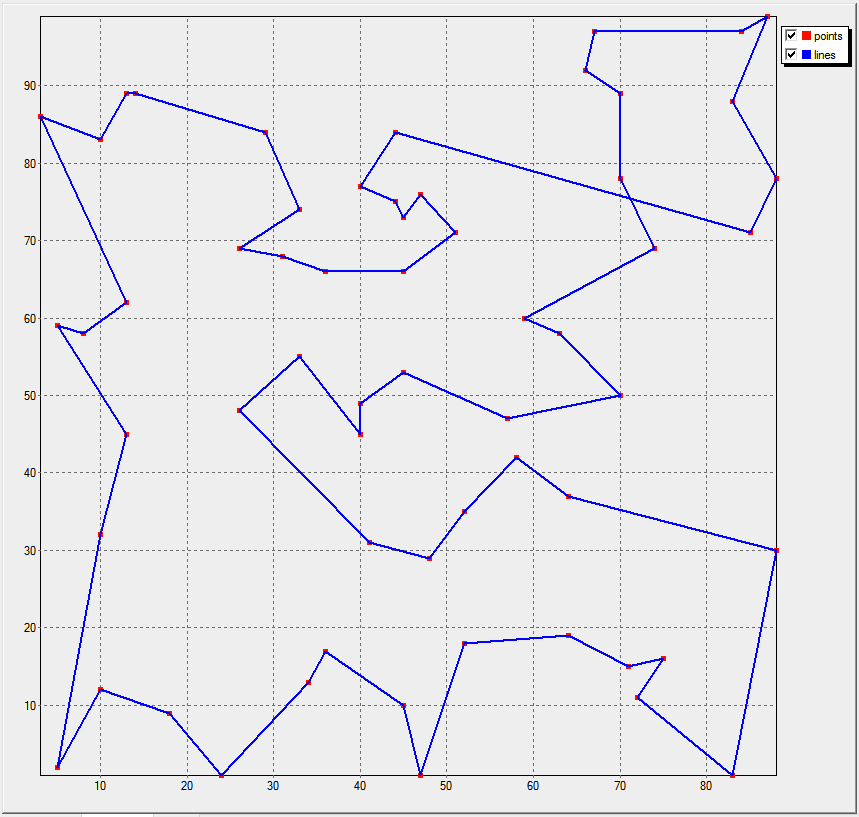
\includegraphics[width=\linewidth]{results-tsp_60_1-grasp}
					\caption{Solución \emph{GRASP}}
				\end{subfigure} \\
				\begin{subfigure}{.4\textwidth}
					\centering
					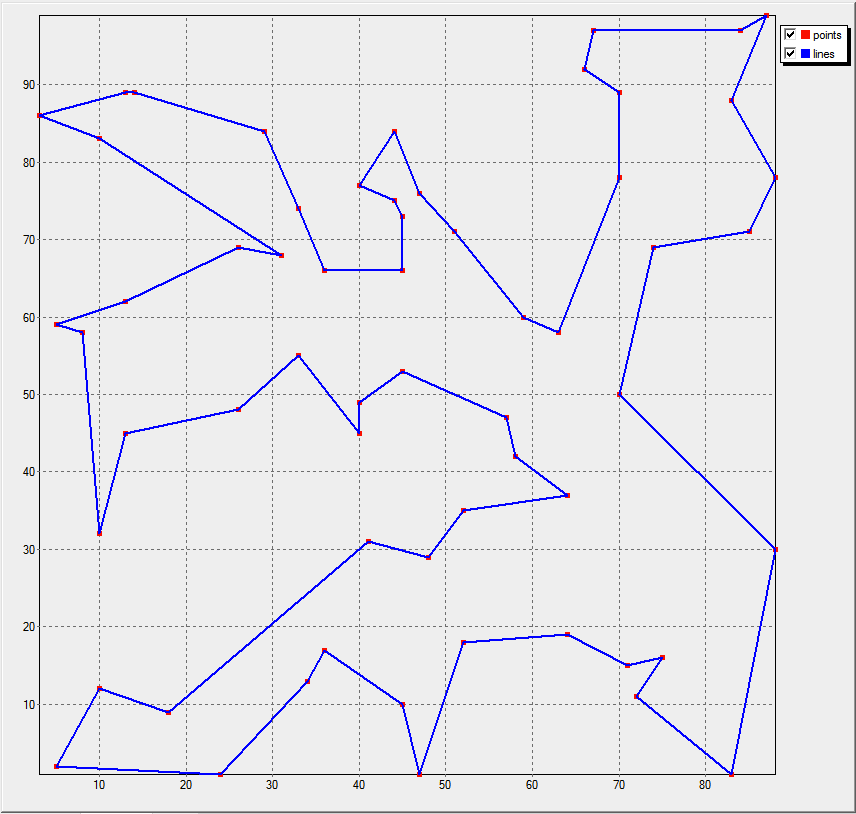
\includegraphics[width=\linewidth]{results-tsp_60_1-sa}
					\caption{Solución \emph{Simulated Anneling}}
				\end{subfigure}
				\caption{Representación gráfica de las distintas soluciones para el conjunto de datos \emph{tsp\_60\_1}}
				\label{fig:sol-tsp_60_1}
			\end{figure}


		\subsection{tsp\_60\_2}

			\paragraph{}
			El conjunto de datos está formado por las coordenadas de $60$ nodos (por lo que es necesario calcular las distancias previamente). En este caso se ha resulto de manera exacta mediante la formulación de \emph{Tucker-Miller} y de manera aproximada mediante heurísticas \emph{Entorno más Cercano}, \emph{2-opt}, \emph{GRASP} y \emph{Simulated Anneling}. En la tabla \ref{table:sol-tsp_60_2} se muestran los resultados de forma numérica mientras que en la figura \ref{fig:sol-tsp_60_2} se muestra la representación gráfica.

			\begin{table}[H]
				\centering
				\begin{tabu}{ | c | c | p{.65\linewidth} |}
					\hline
			   	\bfseries Método & \bfseries Distancia & \bfseries Camino
			    \csvreader[head to column names]{../results/csv/results-tsp_60_2.csv}{}
			    {\\\hline\method&\distance&\path}
					\\\hline
		    \end{tabu}
				\caption{Soluciones para el conjunto de datos \emph{tsp\_60\_2}}
				\label{table:sol-tsp_60_2}
			\end{table}

			\begin{figure}[h]
				\centering
				\begin{subfigure}{.4\textwidth}
					\centering
					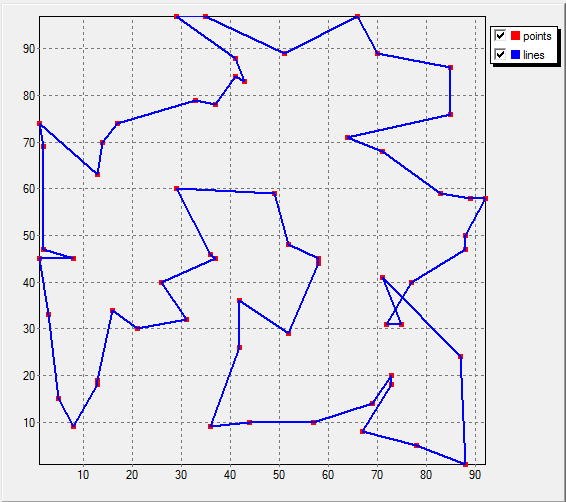
\includegraphics[width=\linewidth]{results-tsp_60_2-exact}
					\caption{Solución \emph{Exacta}}
				\end{subfigure} \
				\begin{subfigure}{.4\textwidth}
					\centering
					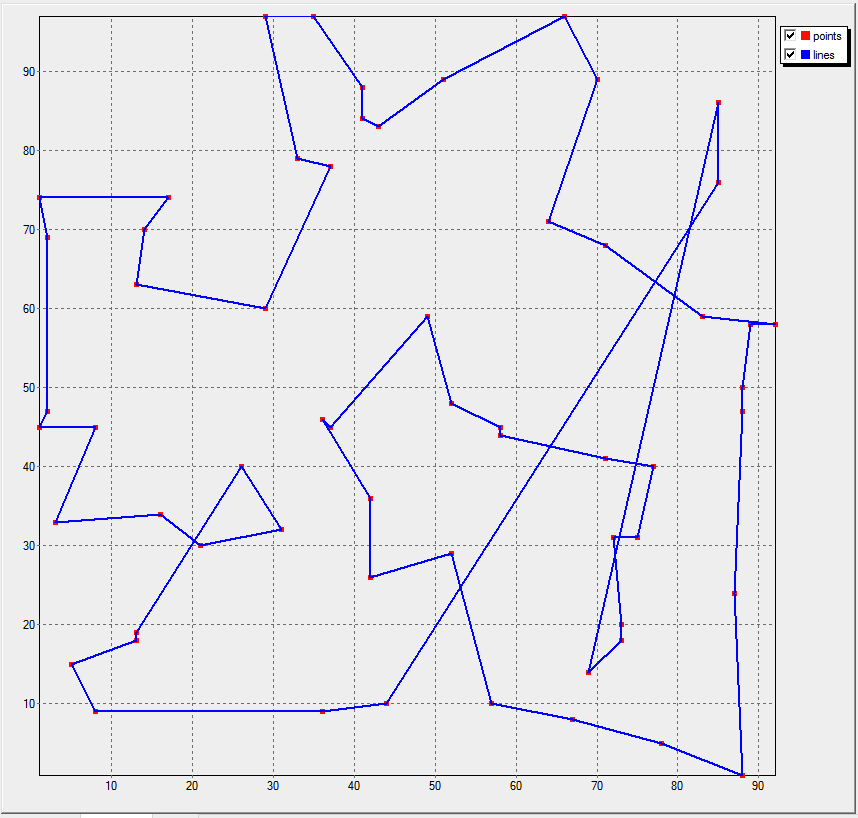
\includegraphics[width=\linewidth]{results-tsp_60_2-greedy}
					\caption{Solución \emph{Entorno más Cercano}}
				\end{subfigure} \\
				\begin{subfigure}{.4\textwidth}
					\centering
					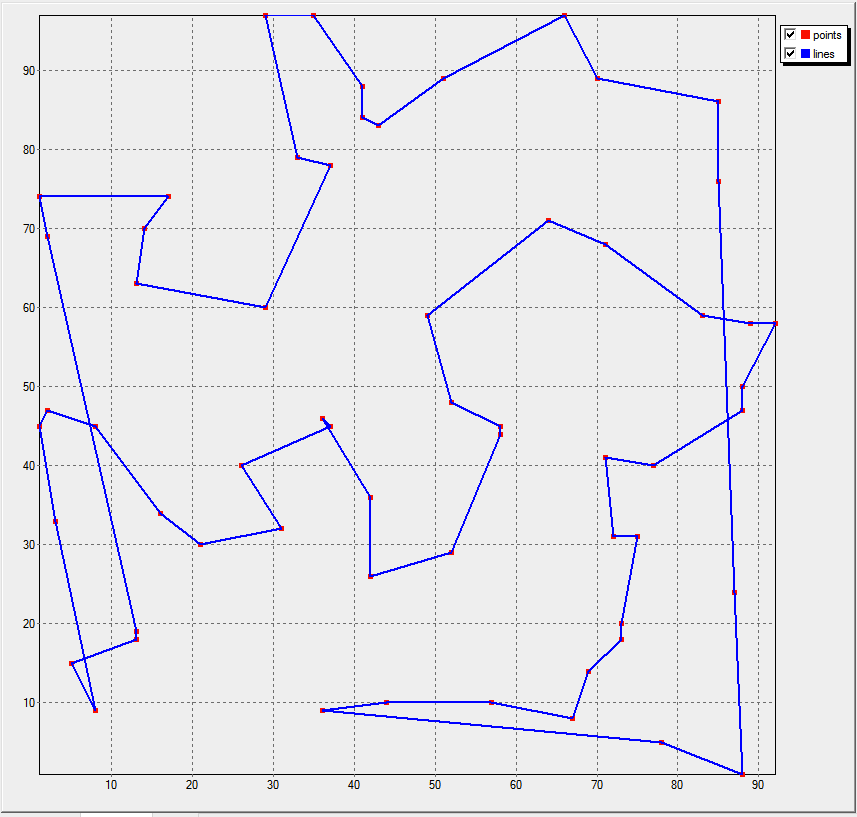
\includegraphics[width=\linewidth]{results-tsp_60_2-opt}
					\caption{Solución \emph{2-opt}}
				\end{subfigure} \
				\begin{subfigure}{.4\textwidth}
					\centering
					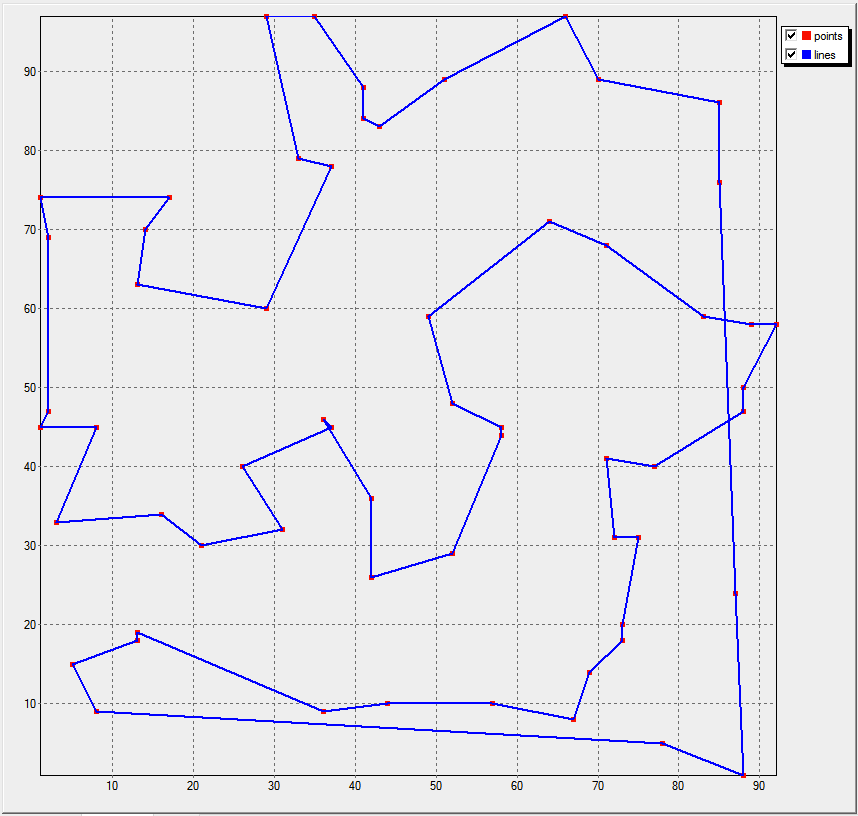
\includegraphics[width=\linewidth]{results-tsp_60_2-grasp}
					\caption{Solución \emph{GRASP}}
				\end{subfigure} \\
				\begin{subfigure}{.4\textwidth}
					\centering
					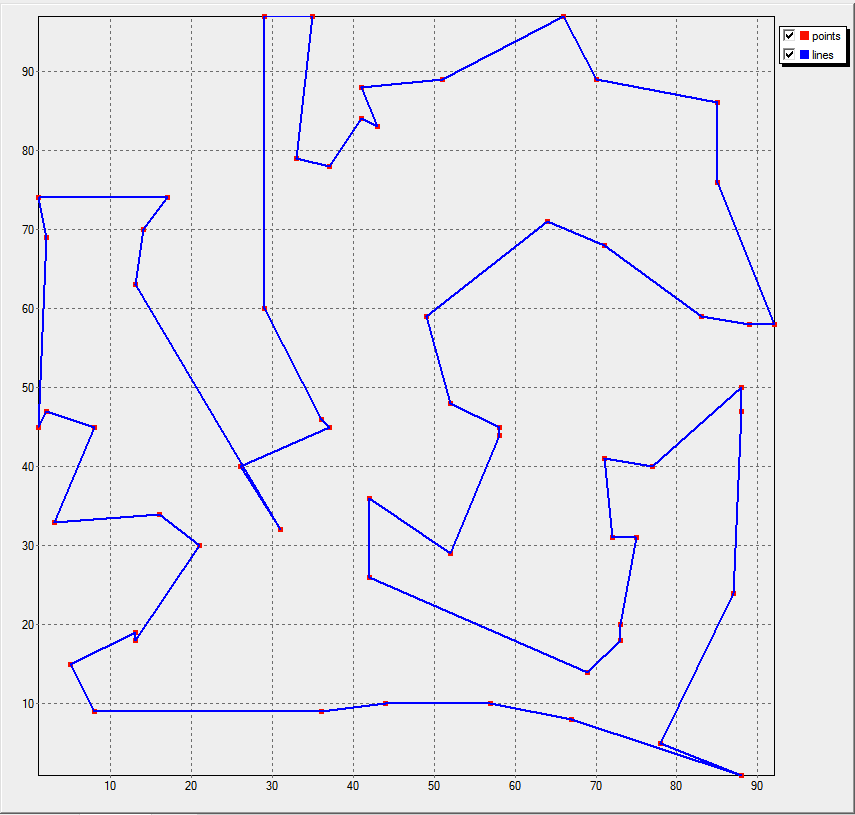
\includegraphics[width=\linewidth]{results-tsp_60_2-sa}
					\caption{Solución \emph{Simulated Anneling}}
				\end{subfigure}
				\caption{Representación gráfica de las distintas soluciones para el conjunto de datos \emph{tsp\_60\_2}}
				\label{fig:sol-tsp_60_2}
			\end{figure}

		\subsection{tsp\_60\_3}

			\paragraph{}
			El conjunto de datos está formado por las coordenadas de $60$ nodos (por lo que es necesario calcular las distancias previamente). En este caso se ha resulto de manera exacta mediante la formulación de \emph{Tucker-Miller} y de manera aproximada mediante heurísticas \emph{Entorno más Cercano}, \emph{2-opt}, \emph{GRASP} y \emph{Simulated Anneling}. En la tabla \ref{table:sol-tsp_60_3} se muestran los resultados de forma numérica mientras que en la figura \ref{fig:sol-tsp_60_3} se muestra la representación gráfica.

			\begin{table}[H]
				\centering
				\begin{tabu}{ | c | c | p{.65\linewidth} |}
					\hline
			   	\bfseries Método & \bfseries Distancia & \bfseries Camino
			    \csvreader[head to column names]{../results/csv/results-tsp_60_3.csv}{}
			    {\\\hline\method&\distance&\path}
					\\\hline
		    \end{tabu}
				\caption{Soluciones para el conjunto de datos \emph{tsp\_60\_3}}
				\label{table:sol-tsp_60_3}
			\end{table}

			\begin{figure}[h]
				\centering
				\begin{subfigure}{.4\textwidth}
					\centering
					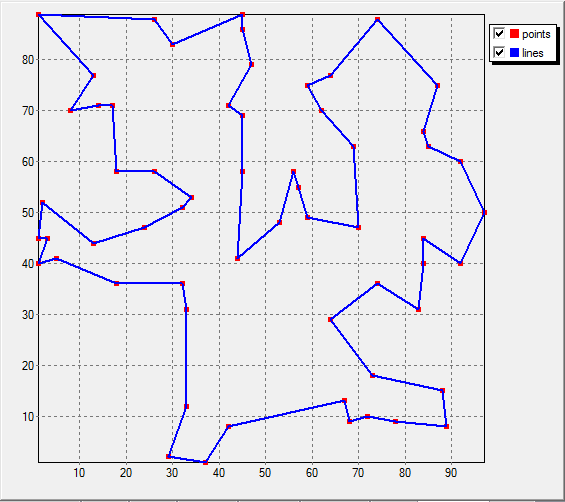
\includegraphics[width=\linewidth]{results-tsp_60_3-exact}
					\caption{Solución \emph{Exacta}}
				\end{subfigure} \
				\begin{subfigure}{.4\textwidth}
					\centering
					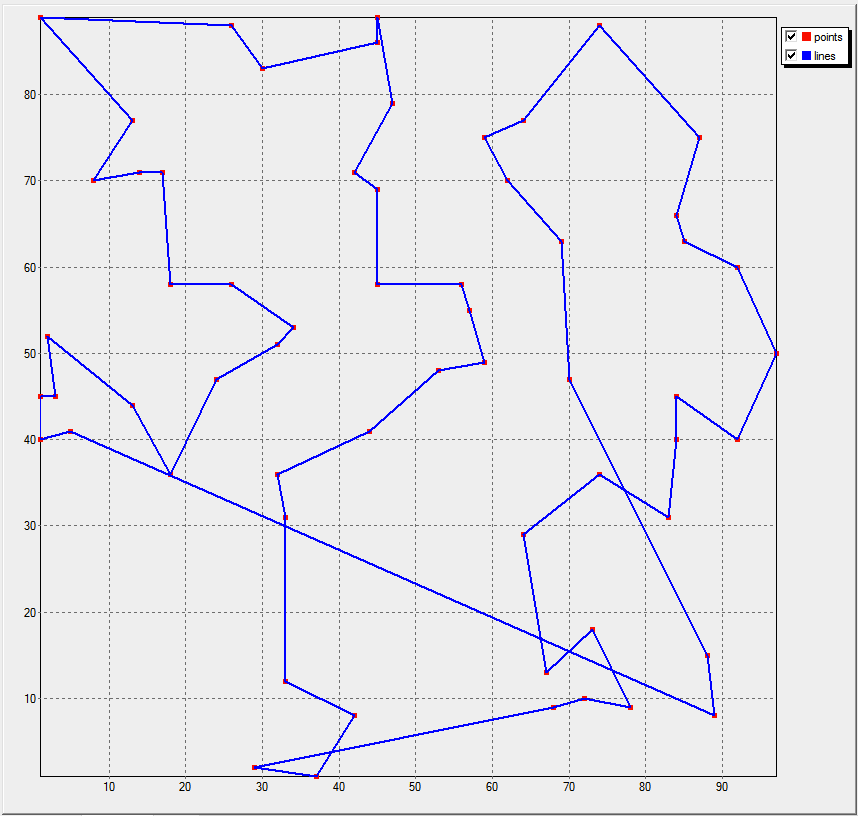
\includegraphics[width=\linewidth]{results-tsp_60_3-greedy}
					\caption{Solución \emph{Entorno más Cercano}}
				\end{subfigure} \\
				\begin{subfigure}{.4\textwidth}
					\centering
					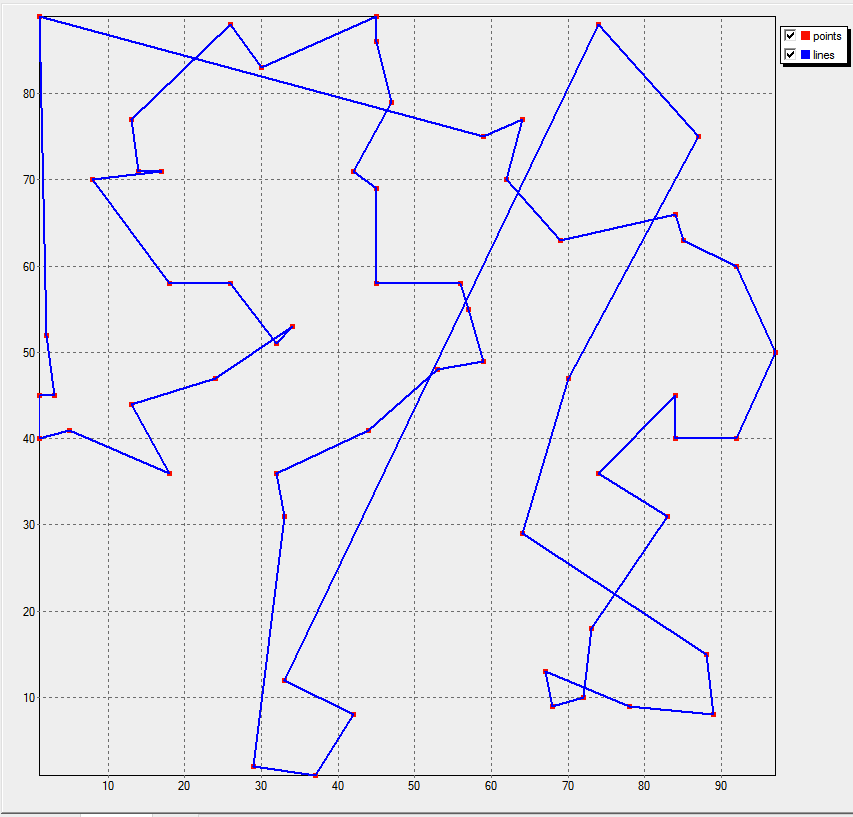
\includegraphics[width=\linewidth]{results-tsp_60_3-opt}
					\caption{Solución \emph{2-opt}}
				\end{subfigure} \
				\begin{subfigure}{.4\textwidth}
					\centering
					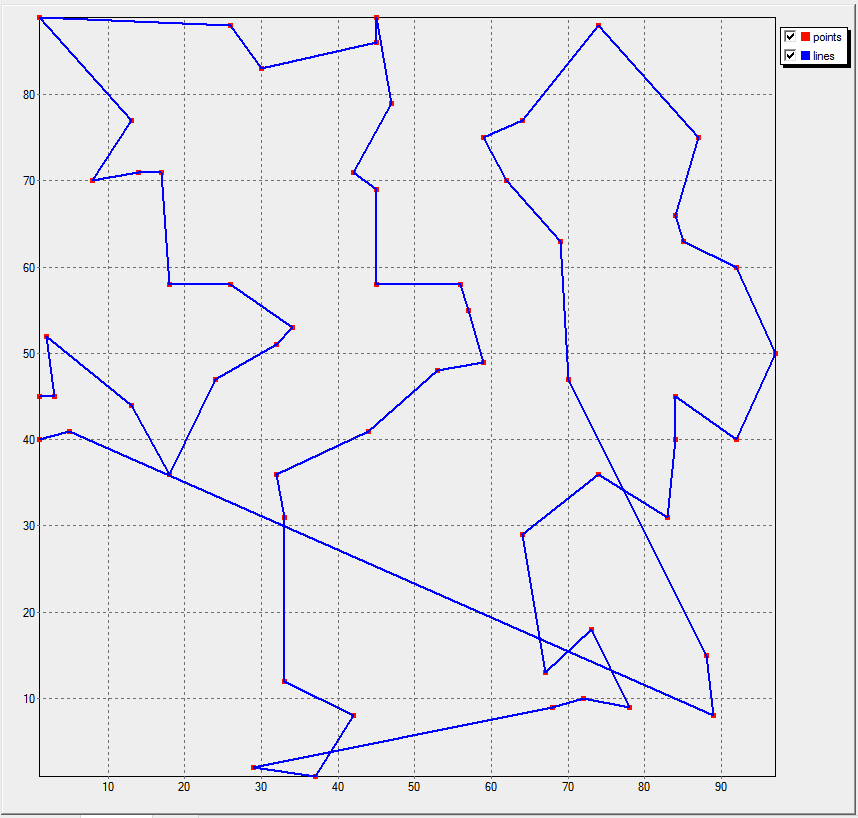
\includegraphics[width=\linewidth]{results-tsp_60_3-grasp}
					\caption{Solución \emph{GRASP}}
				\end{subfigure} \\
				\begin{subfigure}{.4\textwidth}
					\centering
					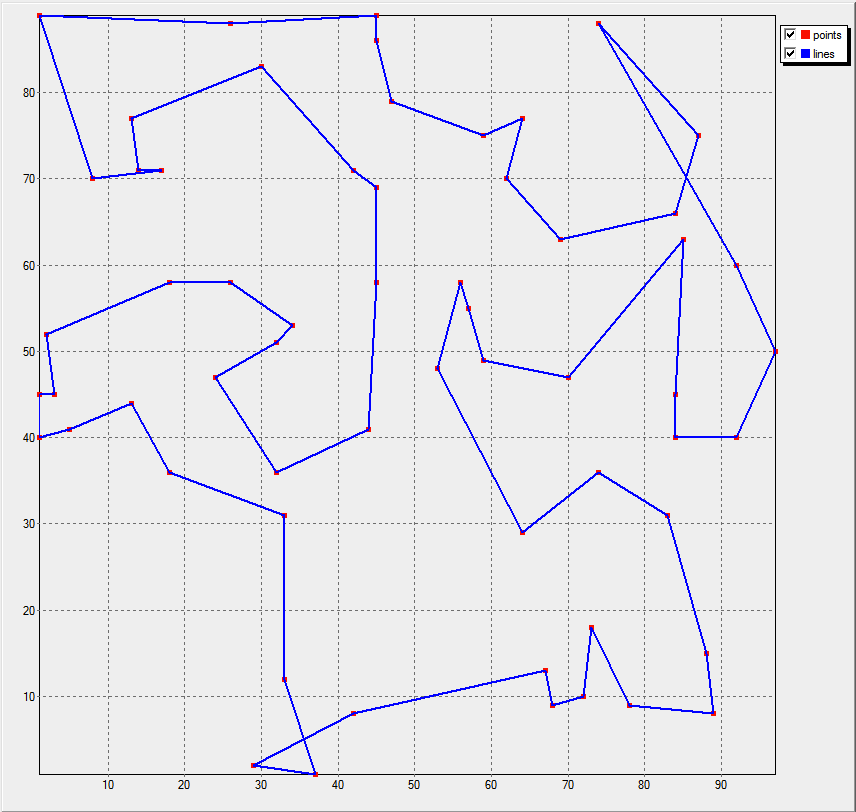
\includegraphics[width=\linewidth]{results-tsp_60_3-sa}
					\caption{Solución \emph{Simulated Anneling}}
				\end{subfigure}
				\caption{Representación gráfica de las distintas soluciones para el conjunto de datos \emph{tsp\_60\_3}}
				\label{fig:sol-tsp_60_3}
			\end{figure}

		\subsection{tsp\_100\_1}

			\paragraph{}
			El conjunto de datos está formado por las coordenadas de $100$ nodos (por lo que es necesario calcular las distancias previamente). En este caso se ha resulto de manera exacta mediante la formulación de \emph{Tucker-Miller} y de manera aproximada mediante heurísticas \emph{Entorno más Cercano}, \emph{2-opt}, \emph{GRASP} y \emph{Simulated Anneling}. En la tabla \ref{table:sol-tsp_100_1} se muestran los resultados de forma numérica mientras que en la figura \ref{fig:sol-tsp_100_1} se muestra la representación gráfica.

			\begin{table}[H]
				\centering
				\begin{tabu}{ | c | c | p{.65\linewidth} |}
					\hline
			   	\bfseries Método & \bfseries Distancia & \bfseries Camino
			    \csvreader[head to column names]{../results/csv/results-tsp_100_1.csv}{}
			    {\\\hline\method&\distance&\path}
					\\\hline
		    \end{tabu}
				\caption{Soluciones para el conjunto de datos \emph{tsp\_100\_1}}
				\label{table:sol-tsp_100_1}
			\end{table}

			\begin{figure}[h]
				\centering
				\begin{subfigure}{.4\textwidth}
					\centering
					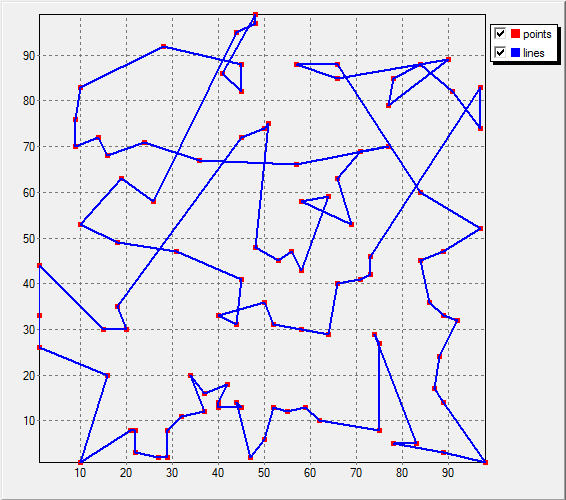
\includegraphics[width=\linewidth]{results-tsp_100_1-exact}
					\caption{Solución \emph{Exacta}}
				\end{subfigure} \
				\begin{subfigure}{.4\textwidth}
					\centering
					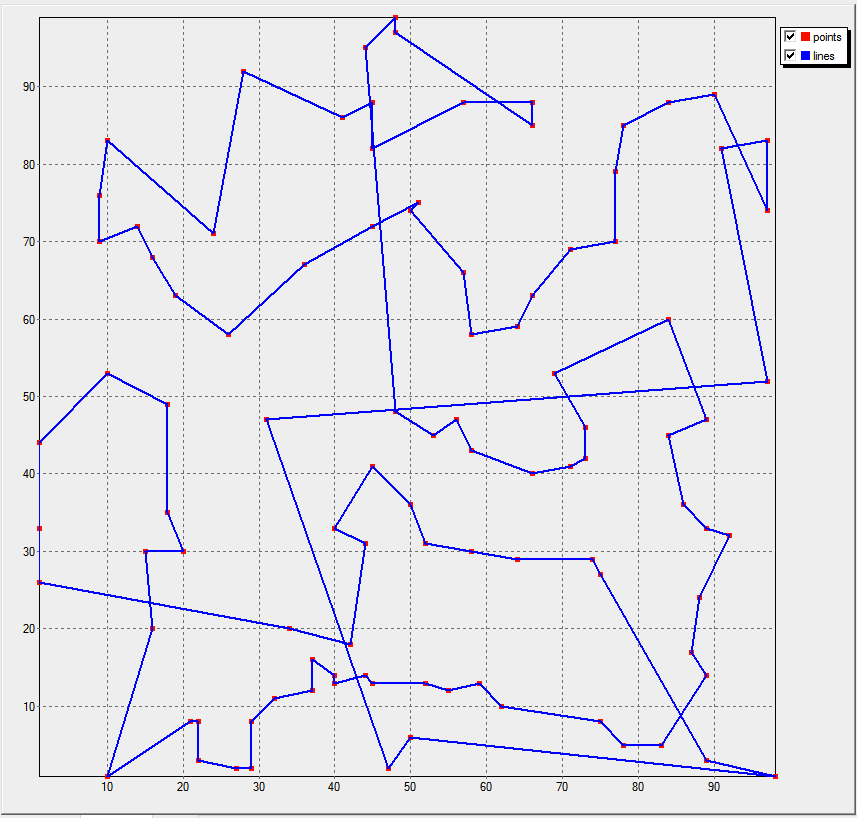
\includegraphics[width=\linewidth]{results-tsp_100_1-greedy}
					\caption{Solución \emph{Entorno más Cercano}}
				\end{subfigure} \\
				\begin{subfigure}{.4\textwidth}
					\centering
					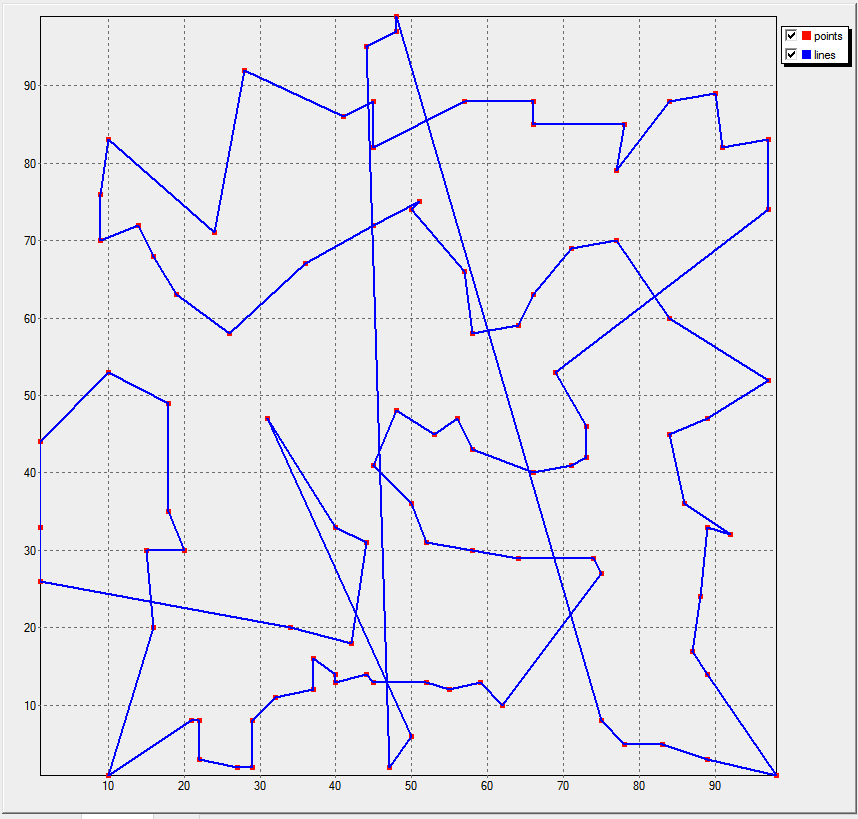
\includegraphics[width=\linewidth]{results-tsp_100_1-opt}
					\caption{Solución \emph{2-opt}}
				\end{subfigure} \
				\begin{subfigure}{.4\textwidth}
					\centering
					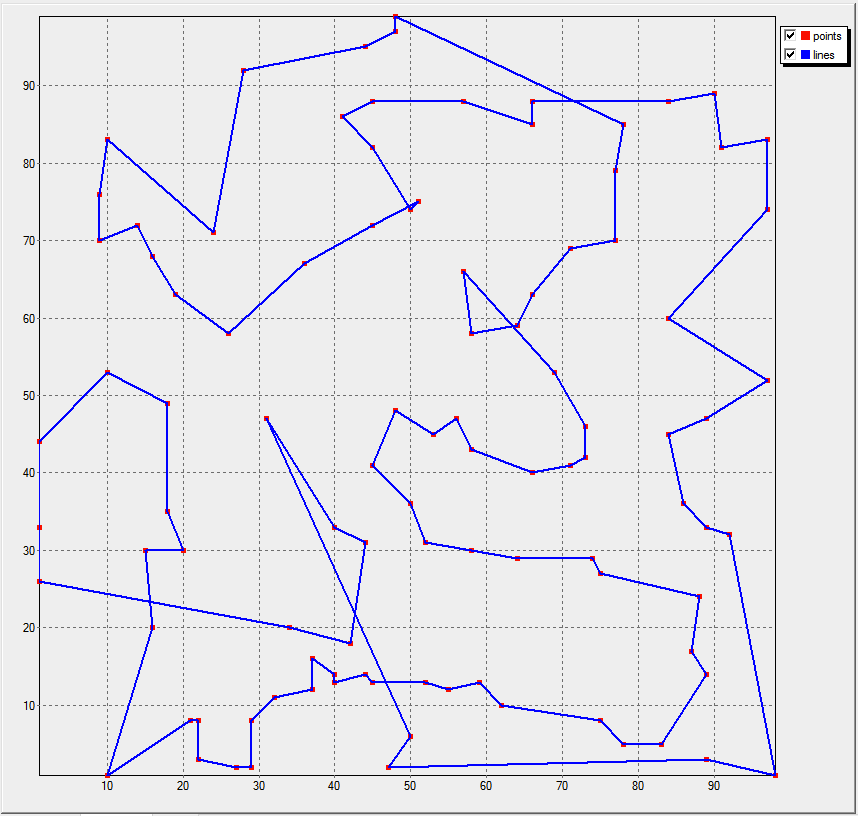
\includegraphics[width=\linewidth]{results-tsp_100_1-grasp}
					\caption{Solución \emph{GRASP}}
				\end{subfigure} \\
				\begin{subfigure}{.4\textwidth}
					\centering
					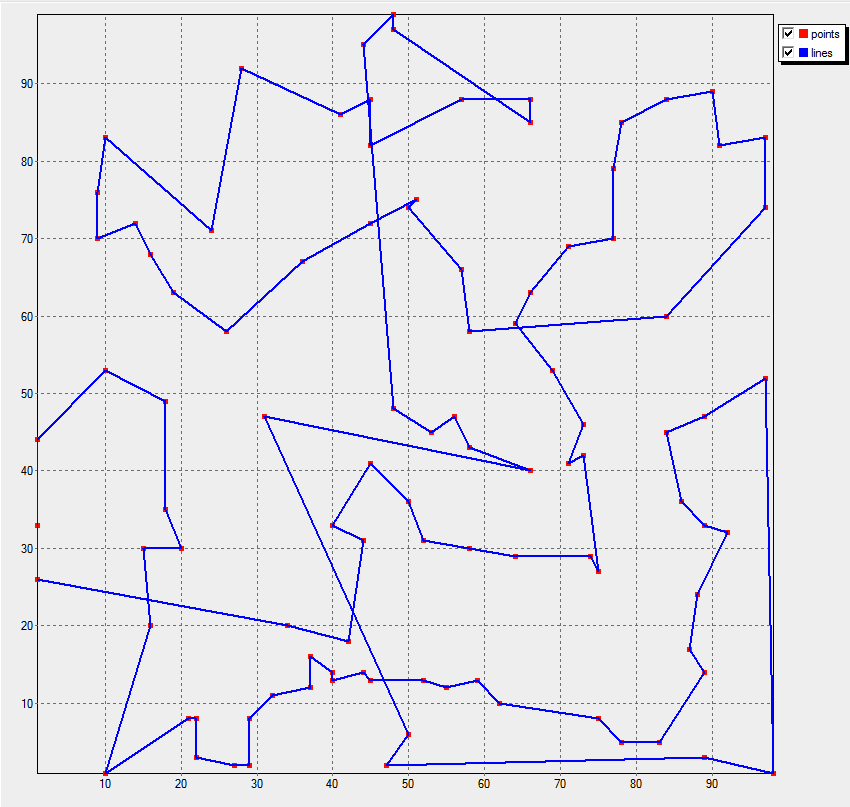
\includegraphics[width=\linewidth]{results-tsp_100_1-sa}
					\caption{Solución \emph{Simulated Anneling}}
				\end{subfigure}
				\caption{Representación gráfica de las distintas soluciones para el conjunto de datos \emph{tsp\_100\_1}}
				\label{fig:sol-tsp_100_1}
			\end{figure}

		\subsection{tsp\_100\_2}

			\paragraph{}
			El conjunto de datos está formado por las coordenadas de $100$ nodos (por lo que es necesario calcular las distancias previamente). En este caso se ha resulto de manera exacta mediante la formulación de \emph{Tucker-Miller} y de manera aproximada mediante heurísticas \emph{Entorno más Cercano}, \emph{2-opt}, \emph{GRASP} y \emph{Simulated Anneling}. En la tabla \ref{table:sol-tsp_100_2} se muestran los resultados de forma numérica mientras que en la figura \ref{fig:sol-tsp_100_2} se muestra la representación gráfica.

			\begin{table}[H]
				\centering
				\begin{tabu}{ | c | c | p{.65\linewidth} |}
					\hline
					\bfseries Método & \bfseries Distancia & \bfseries Camino
					\csvreader[head to column names]{../results/csv/results-tsp_100_2.csv}{}
					{\\\hline\method&\distance&\path}
					\\\hline
				\end{tabu}
				\caption{Soluciones para el conjunto de datos \emph{tsp\_100\_2}}
				\label{table:sol-tsp_100_2}
			\end{table}

			\begin{figure}[h]
				\centering
				\begin{subfigure}{.4\textwidth}
					\centering
					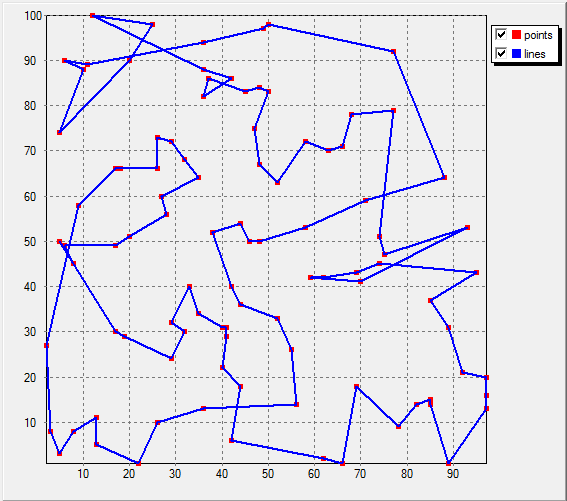
\includegraphics[width=\linewidth]{results-tsp_100_2-exact}
					\caption{Solución \emph{Exacta}}
				\end{subfigure} \
				\begin{subfigure}{.4\textwidth}
					\centering
					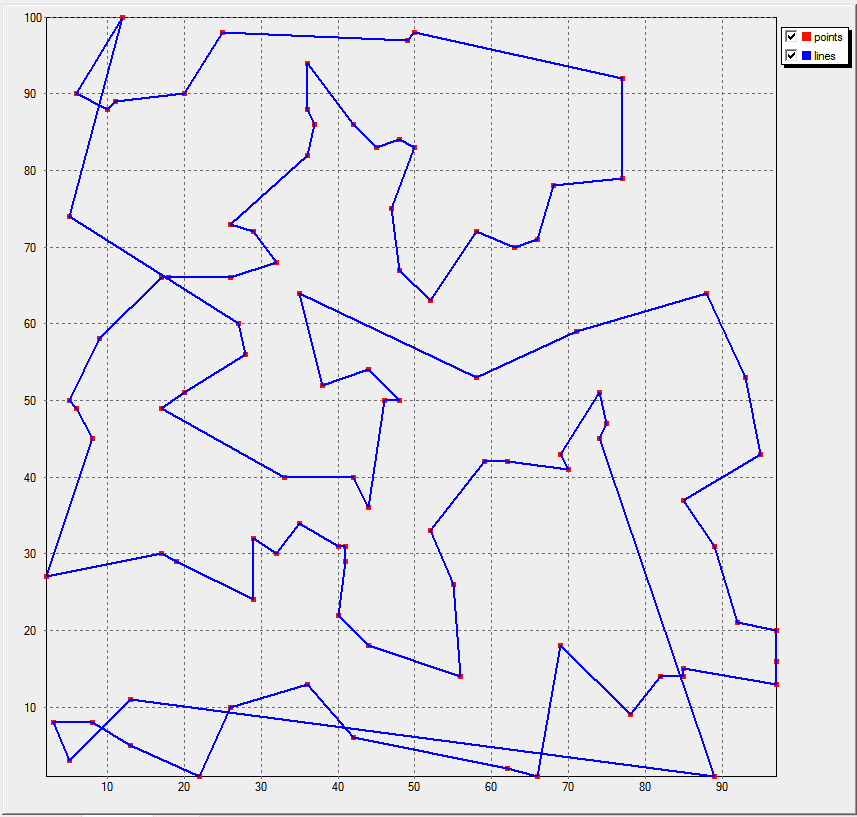
\includegraphics[width=\linewidth]{results-tsp_100_2-greedy}
					\caption{Solución \emph{Entorno más Cercano}}
				\end{subfigure} \\
				\begin{subfigure}{.4\textwidth}
					\centering
					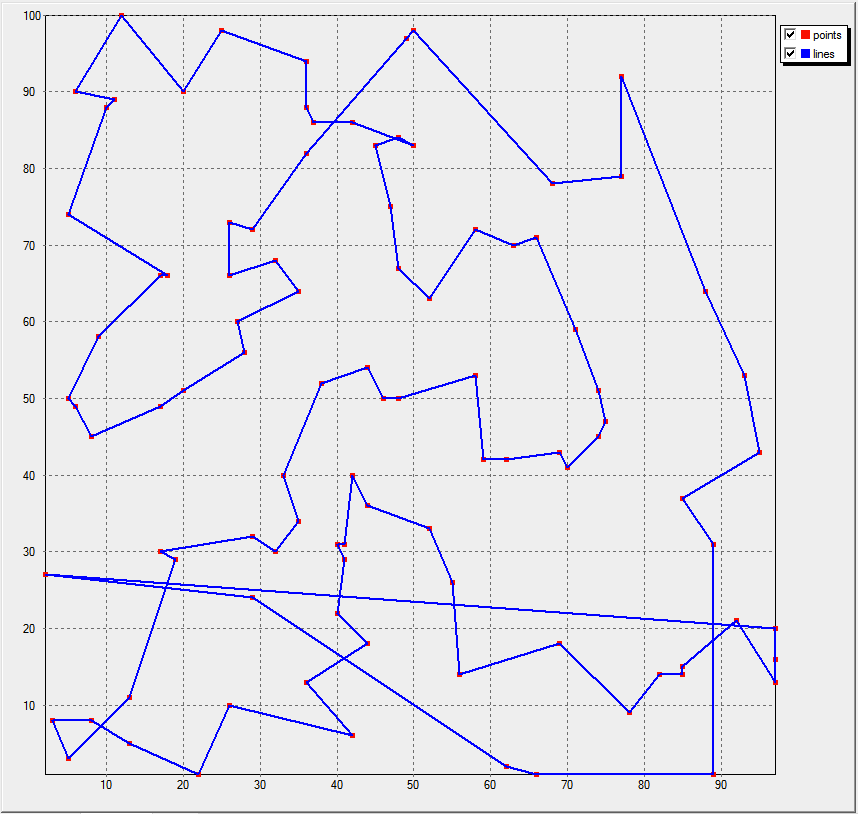
\includegraphics[width=\linewidth]{results-tsp_100_2-opt}
					\caption{Solución \emph{2-opt}}
				\end{subfigure} \
				\begin{subfigure}{.4\textwidth}
					\centering
					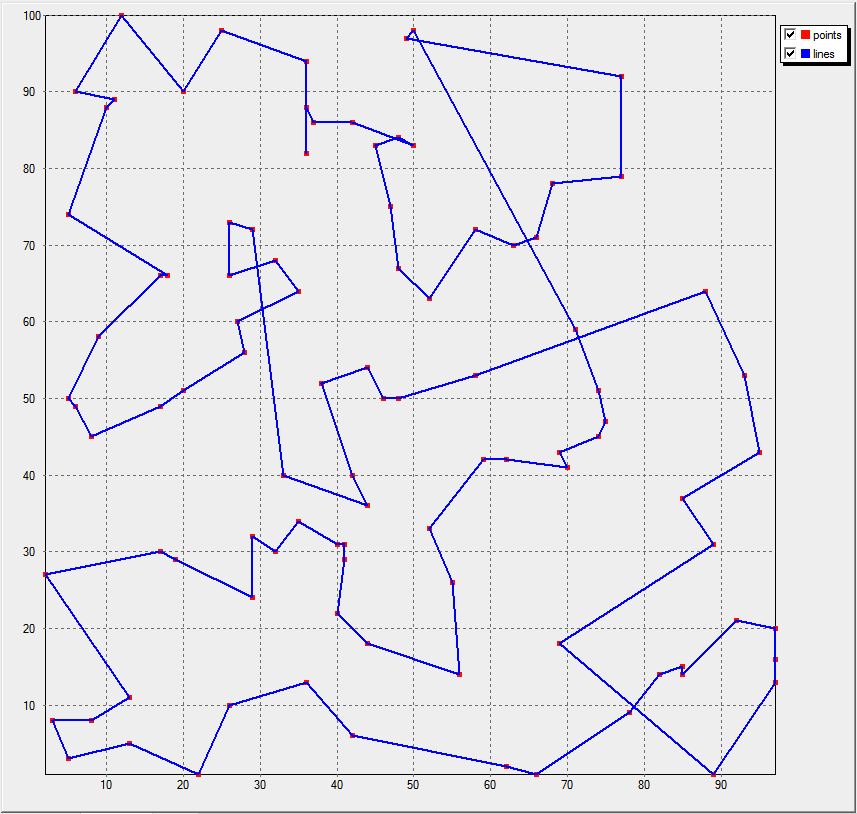
\includegraphics[width=\linewidth]{results-tsp_100_2-grasp}
					\caption{Solución \emph{GRASP}}
				\end{subfigure} \\
				\begin{subfigure}{.4\textwidth}
					\centering
					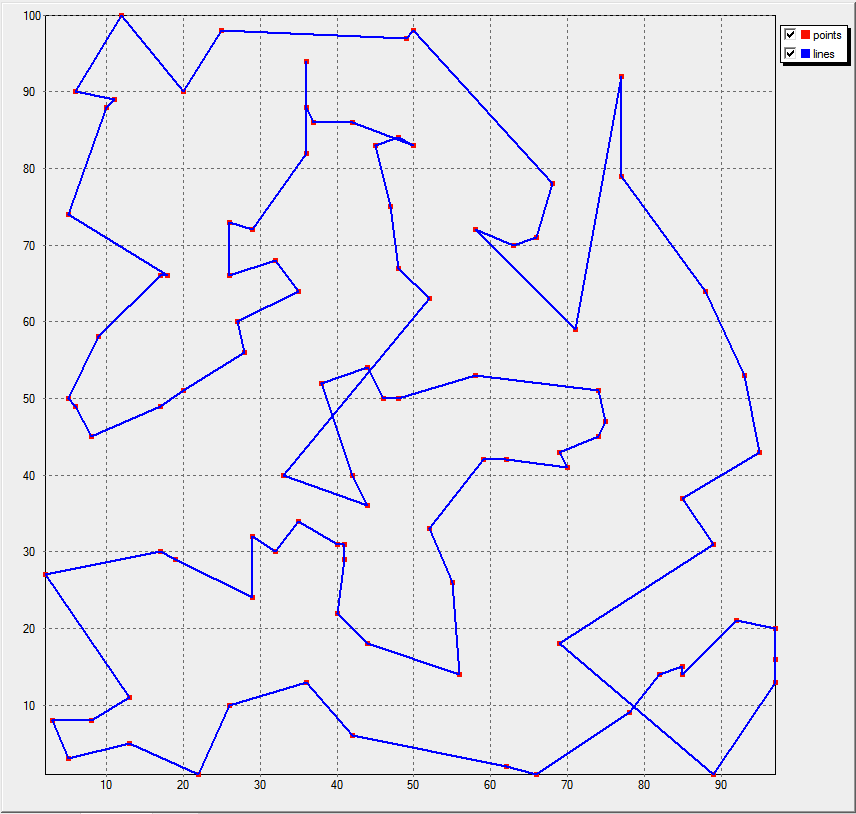
\includegraphics[width=\linewidth]{results-tsp_100_2-sa}
					\caption{Solución \emph{Simulated Anneling}}
				\end{subfigure}
				\caption{Representación gráfica de las distintas soluciones para el conjunto de datos \emph{tsp\_100\_2}}
				\label{fig:sol-tsp_100_2}
			\end{figure}

		\subsection{tsp\_100\_3}

			\paragraph{}
			El conjunto de datos está formado por las coordenadas de $100$ nodos (por lo que es necesario calcular las distancias previamente). En este caso se ha resulto de manera exacta mediante la formulación de \emph{Tucker-Miller} y de manera aproximada mediante heurísticas \emph{Entorno más Cercano}, \emph{2-opt}, \emph{GRASP} y \emph{Simulated Anneling}. En la tabla \ref{table:sol-tsp_100_3} se muestran los resultados de forma numérica mientras que en la figura \ref{fig:sol-tsp_100_3} se muestra la representación gráfica.

			\begin{table}[H]
				\centering
				\begin{tabu}{ | c | c | p{.65\linewidth} |}
					\hline
					\bfseries Método & \bfseries Distancia & \bfseries Camino
					\csvreader[head to column names]{../results/csv/results-tsp_100_3.csv}{}
					{\\\hline\method&\distance&\path}
					\\\hline
				\end{tabu}
				\caption{Soluciones para el conjunto de datos \emph{tsp\_100\_3}}
				\label{table:sol-tsp_100_3}
			\end{table}

			\begin{figure}[h]
				\centering
				\begin{subfigure}{.4\textwidth}
					\centering
					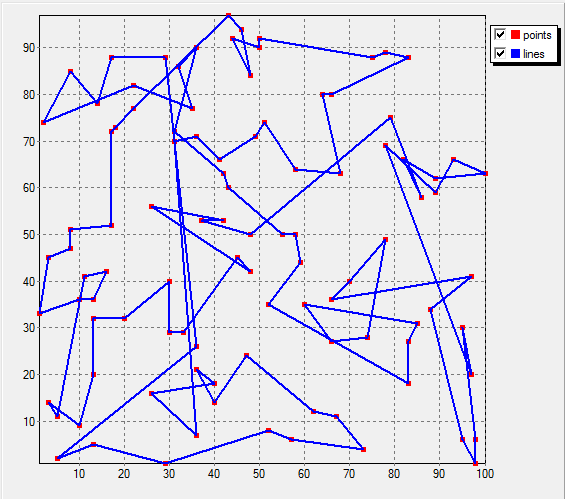
\includegraphics[width=\linewidth]{results-tsp_100_3-exact}
					\caption{Solución \emph{Exacta}}
				\end{subfigure} \
				\begin{subfigure}{.4\textwidth}
					\centering
					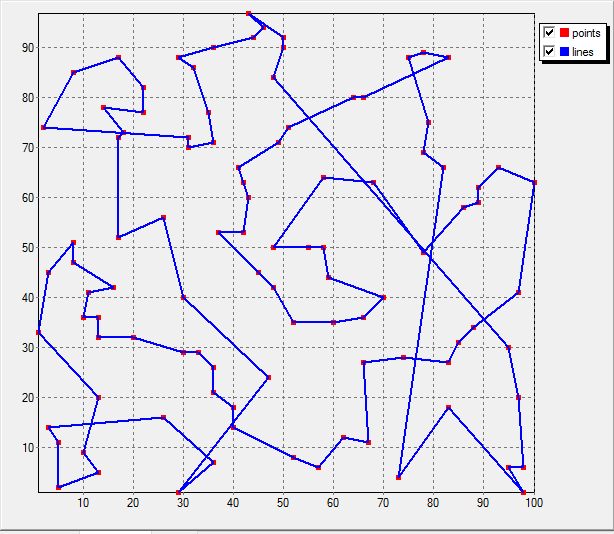
\includegraphics[width=\linewidth]{results-tsp_100_3-greedy}
					\caption{Solución \emph{Entorno más Cercano}}
				\end{subfigure} \\
				\begin{subfigure}{.4\textwidth}
					\centering
					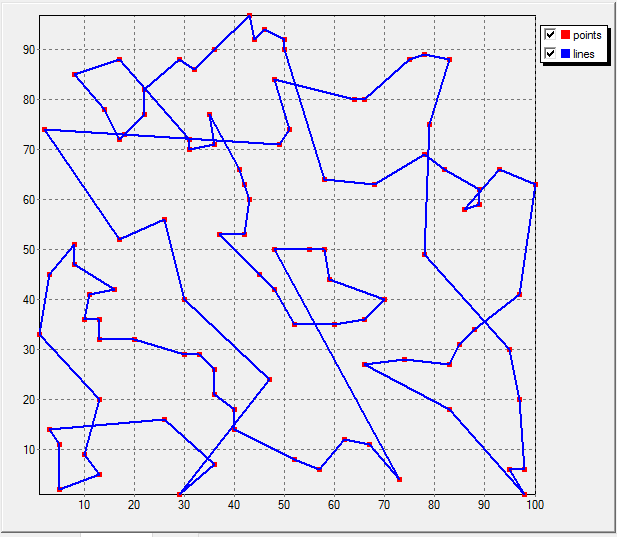
\includegraphics[width=\linewidth]{results-tsp_100_3-opt}
					\caption{Solución \emph{2-opt}}
				\end{subfigure} \
				\begin{subfigure}{.4\textwidth}
					\centering
					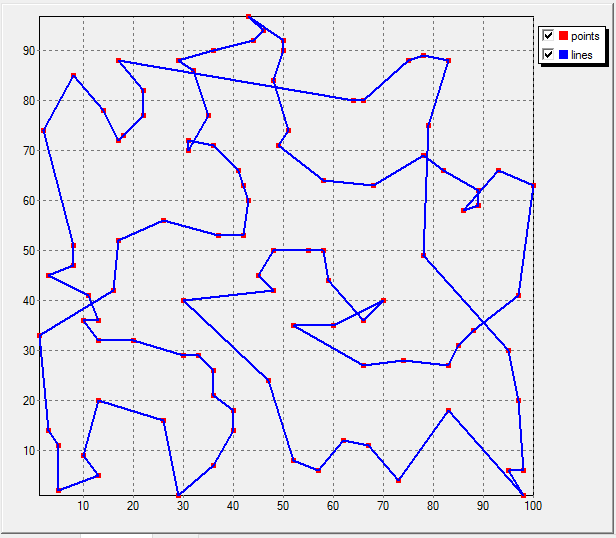
\includegraphics[width=\linewidth]{results-tsp_100_3-grasp}
					\caption{Solución \emph{GRASP}}
				\end{subfigure} \\
				\begin{subfigure}{.4\textwidth}
					\centering
					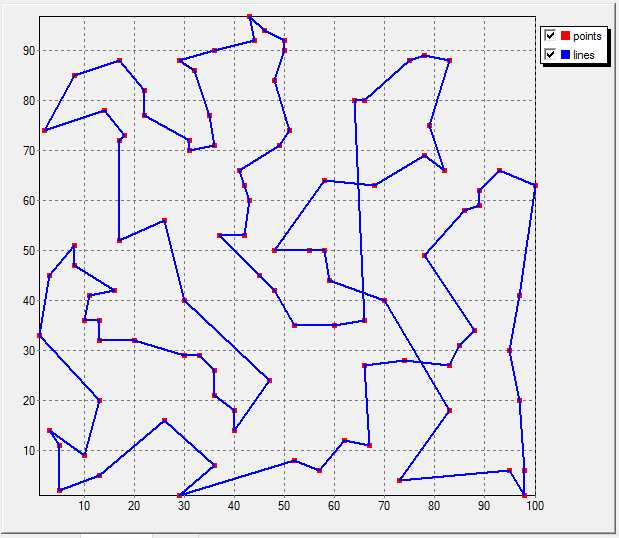
\includegraphics[width=\linewidth]{results-tsp_100_3-sa}
					\caption{Solución \emph{Simulated Anneling}}
				\end{subfigure}
				\caption{Representación gráfica de las distintas soluciones para el conjunto de datos \emph{tsp\_100\_3}}
				\label{fig:sol-tsp_100_3}
			\end{figure}

		\subsection{n40w20.001}

			\paragraph{}
			El conjunto de datos está formado por la matriz de distancias de $41$ nodos junto con sus correspondientes ventanas de tiempo. En este caso se ha resulto de manera exacta mediante la formulación de \emph{Tucker-Miller} añadiendo las correspondientes restricciones \emph{beta}($\beta$) referidas a las ventanas de tiempo. Los resultados se muestran en la tabla \ref{table:sol-n40w20.001}.

			\begin{table}[H]
				\centering
				\begin{tabu}{ | c | c | p{.65\linewidth} |}
					\hline
			   	\bfseries Método & \bfseries Distancia & \bfseries Camino
			    \csvreader[head to column names]{../results/csv/results-n40w20.001.csv}{}
			    {\\\hline\method&\distance&\path}
					\\\hline
		    \end{tabu}
				\caption{Soluciones para el conjunto de datos \emph{n40w20.001}}
				\label{table:sol-n40w20.001}
			\end{table}

		\subsection{n40w20.004}

			\paragraph{}
			El conjunto de datos está formado por la matriz de distancias de $41$ nodos junto con sus correspondientes ventanas de tiempo. En este caso se ha resulto de manera exacta mediante la formulación de \emph{Tucker-Miller} añadiendo las correspondientes restricciones \emph{beta}($\beta$) referidas a las ventanas de tiempo. Los resultados se muestran en la tabla \ref{table:sol-n40w20.004}.

			\begin{table}[H]
				\centering
				\begin{tabu}{ | c | c | p{.65\linewidth} |}
					\hline
			   	\bfseries Método & \bfseries Distancia & \bfseries Camino
			    \csvreader[head to column names]{../results/csv/results-n40w20.004.csv}{}
			    {\\\hline\method&\distance&\path}
					\\\hline
		    \end{tabu}
				\caption{Soluciones para el conjunto de datos \emph{n40w20.004}}
				\label{table:sol-n40w20.004}
			\end{table}

		\subsection{n60w20.005}

			\paragraph{}
			El conjunto de datos está formado por la matriz de distancias de $61$ nodos junto con sus correspondientes ventanas de tiempo. En este caso se ha resulto de manera exacta mediante la formulación de \emph{Tucker-Miller} añadiendo las correspondientes restricciones \emph{beta}($\beta$) referidas a las ventanas de tiempo. Los resultados se muestran en la tabla \ref{table:sol-n60w20.005}.

			\begin{table}[H]
				\centering
				\begin{tabu}{ | c | c | p{.65\linewidth} |}
					\hline
			   	\bfseries Método & \bfseries Distancia & \bfseries Camino
			    \csvreader[head to column names]{../results/csv/results-n60w20.005.csv}{}
			    {\\\hline\method&\distance&\path}
					\\\hline
		    \end{tabu}
				\caption{Soluciones para el conjunto de datos \emph{n60w20.005}}
				\label{table:sol-n60w20.005}
			\end{table}


%-----------------------------
%	BIBLIOGRAPHY
%-----------------------------
	\nocite{subject:mio}
	\nocite{garciparedes:mosel-examples}
	\bibliographystyle{acm}
  \bibliography{bib/misc}

\end{document}
